\setAuthor{Tundmatu autor}
\setRound{lõppvoor}
\setYear{2007}
\setNumber{G 5}
\setDifficulty{8}
\setTopic{Kinemaatika}

\prob{Laev}
Maailmas leidub jõgesid, kus vesi tõusude tõttu liigub kord ühes, kord teises suunas. Vaatleme laevaliiklust ühel sellisel jõel. Joonisel on antud vee liikumiskiiruse sõltuvus kellaajast. Positiivseks loetakse vee kiirus siis, kui see on suunatud punktist $A$ punkti $B$ poole. Leida optimaalne (lühimate sõiduaegadega) tunniplaan kaubalaeva regulaarseks liikumiseks üks kord päevas punktist $A$ punkti $B$ ja tagasi. Kaugus nende punktide vahel piki jõge on $L = \SI{20}{km}$, laeva kiirus seisvas vees $v_0 = \SI{4}{km/h}$.

\begin{center}
	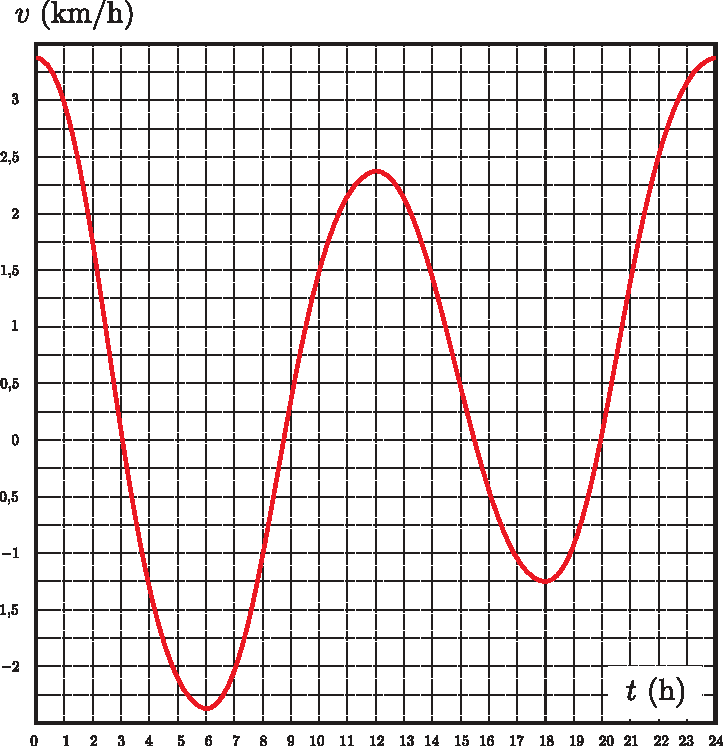
\includegraphics[width=0.7\linewidth]{2007-v3g-05-yl}
\end{center}

\hint
Liikudes $B$ suunas on laeva kiirus $v_0 + v(t)$ ning liikudes $A$ suunas on kiirus $-v_0 + v(t)$. Võimalik on näidata, et kahe punkti vahelise sõiduaja minimeerimiseks peavad voolukiirused alguses ja lõpus olema võrdsed. Vastasel juhul saaks valida veel väiksema sõiduajaga plaani nihutades stardiaega emmas-kummas suunas.

\solu
Näitame, et laev peab sõitma nii, et voolukiirused stardihetkel $t_s$ ja finišihetkel $t_f$ on võrdsed, $v(t_s) = v(t_f)$. Teeme seda vastuväiteliselt. Vaatleme konkreetsuse mõttes liikumist $B$ suunas, mil laeva kiirus kalda suhtes on $v_0 + v(t)$. Sellisel juhul on läbitud vahemaa $L$ graafiku $v(t)$ ja joone $v = -v_0$ vahelise piirkonna pindala. Nihutame stardi ja finišiaega väikese ajavahemiku $\Delta t$ võrra. Läbitav vahemaa muutub seejuures $\Delta t(v_f - v_s)$ võrra. Kui $v(t_s) \neq v(t_f)$, siis saame valida $\Delta t$ märgi selliselt, et $\Delta t(v_f - v_s) > 0$, st sama aja jooksul läbitud vahemaa kasvab saades suuremaks $L$st. Seega saaks sõiduaega vähendada ning stardihetk polnud optimaalne.

Eelpool selgitatud tingimustele (stardi- ja finišihetke kiirused on võrdsed, graafiku ja joone $v = -v_0$ vaheline pindala võrdub \SI{20}{km}-ga) vastavad stardiajad punktist $A$ 22.20 ja punktist $B$ 04.20.
\probend